\documentclass[tikz, border=0mm]{standalone}
\usetikzlibrary{calc}
\newcommand{\tikzsetnextfilename}[1]{}


% One style for all polyomino outlines (adjust to taste)
\tikzset{
  polyoutline/.style={draw=black, line width=2pt}
}

% (3): horizontal bar of length 3
% cells: (0,0), (1,0), (2,0)
\newcommand{\shapeH}[2]{%
  \begin{scope}[shift={(#1,#2)}]
    \draw[polyoutline]
      (0,0) -- (3,0) -- (3,1) -- (0,1) -- cycle;
  \end{scope}%
}

% (1,1,1): vertical bar of length 3
% cells: (0,0), (0,1), (0,2)
\newcommand{\shapeI}[2]{%
  \begin{scope}[shift={(#1,#2)}]
    \draw[polyoutline]
      (0,1) -- (1,1) -- (1,-2) -- (0,-2) -- cycle;
  \end{scope}%
}

% (2,1): hook shape
% cells: (0,0), (1,0), (0,1)
\newcommand{\shapeL}[2]{%
  \begin{scope}[shift={(#1,#2)}]
    \draw[polyoutline]
      (0,-1) -- (2,-1) -- (2,0) -- (1,0) -- (1,1) -- (0,1) -- cycle;
  \end{scope}%
}

% (2,2)/(1): skew shape
% cells: (0,0), (1,0), (1,1)
\newcommand{\shapeS}[2]{%
  \begin{scope}[shift={(#1,#2)}]
    \draw[polyoutline]
      (0,1) -- (2,1) -- (2,-1) -- (1,-1) -- (1,0) -- (0,0) -- cycle;
  \end{scope}%
}


\begin{document}

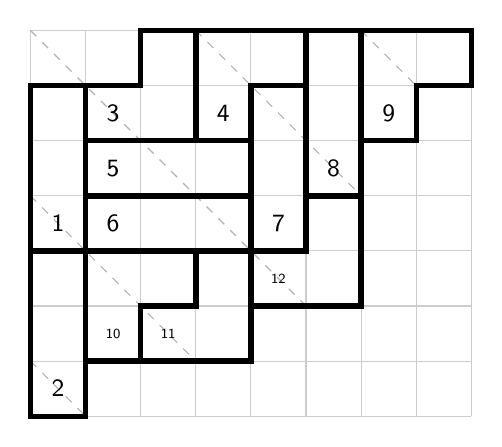
\begin{tikzpicture}[xscale=0.7,yscale=-0.7]

  % --- styles ---
  \tikzset{
    gridbg/.style={draw=gray!40, line width=0.4pt},
    trioutline/.style={draw=black, line width=1.2pt},
    diag/.style={draw=gray!60, dashed},
  }

  % --- background & grid ---
   \draw[step=1,gridbg] (0,0) grid (8,7);

  % =========================
  %  OPTIONAL DIAGONALS
  % =========================

  \draw[diag] (0,0) -- (5,5);
  \draw[diag] (0,3) -- (3,6);
  \draw[diag] (0,6) -- (1,7);
  \draw[diag] (3,0) -- (6,3);
  \draw[diag] (6,0) -- (7,1);




  % =========================
  %  OUTLINED POLYOMINOES
  % =========================

    \shapeI{0}{3}
    \shapeI{0}{6}
    \shapeS{1}{1}
    \shapeL{3}{1}
    \shapeH{1}{2}
    \shapeH{1}{3}
    \shapeI{4}{3}
    \shapeI{5}{2}
    \shapeL{6}{1}
    \shapeL{1}{5}
    \shapeS{2}{5}
    \shapeS{4}{4}

\begin{scope}[shift={(0.5,0.5)}]
  \node[font=\sffamily\small] at (0,3) {1};
  \node[font=\sffamily\small] at (0,6) {2};

  \node[font=\sffamily\small] at (1,1) {3};
  \node[font=\sffamily\small] at (3,1) {4};

  \node[font=\sffamily\small] at (1,2) {5};
  \node[font=\sffamily\small] at (1,3) {6};

  \node[font=\sffamily\small] at (4,3) {7};
  \node[font=\sffamily\small] at (5,2) {8};
  \node[font=\sffamily\small] at (6,1) {9};

  \node[font=\sffamily\tiny]  at (1,5) {10};
  \node[font=\sffamily\tiny]  at (2,5) {11};
  \node[font=\sffamily\tiny]  at (4,4) {12};
\end{scope}

\end{tikzpicture}



\end{document}
